\chapter{Konstruktion}
Für die Konstruktion des \textit{EarthROVERs} wurden drei \textit{Mindstorms education} Kästen und ein \textit{Zusatzkasten} verwendet. Des Weiteren wurden einige HiTechnic Sensoren verwendet.

\section{Basis}
Die Basis trägt alle Teile des \textit{EarthROVERs}, daher muss sie relativ groß sein und möglichst stabil. Bei der Basis haben wir uns für eine flache Konstruktion entschieden.

\begin{capfigure}[Basis]
	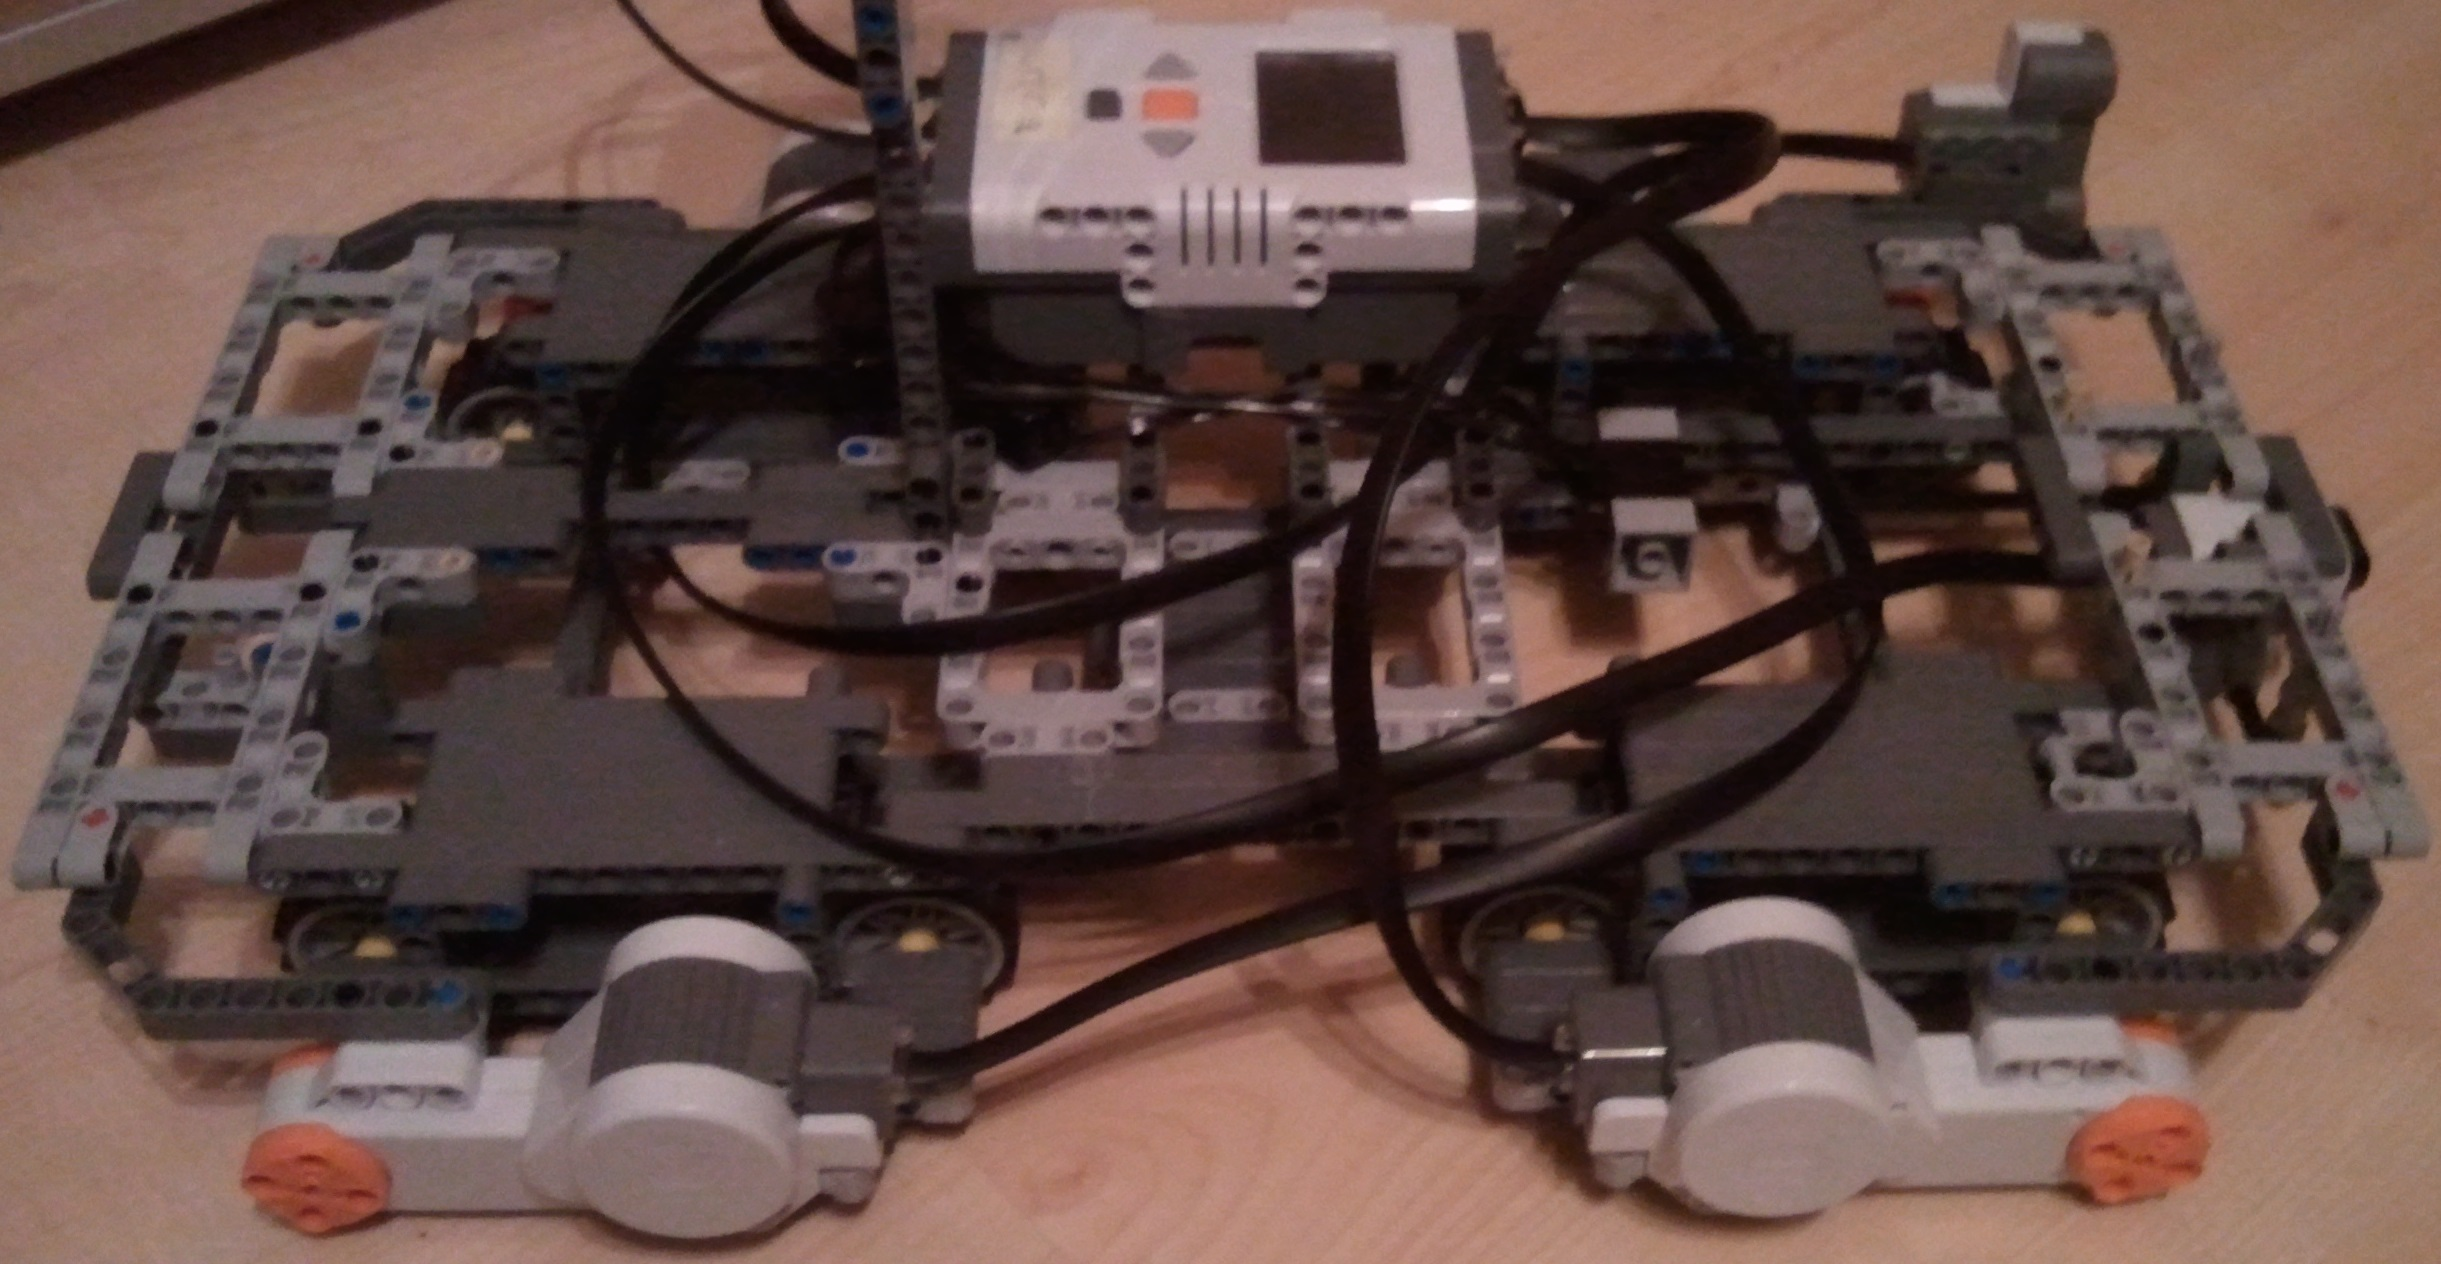
\includegraphics[width=\textwidth]{images/construction/basis/basis}
\end{capfigure}

Auf der Abbildung ist die Basis mit einem der \textit{NXT-Bricks}, dem \nameref{cha:fahrwerk} und den \nameref{cha:sensoren} 

\subsection{Sensorturm}
Für den \textit{HiTechnic Compass Sensor} und den \textit{HiTechnic Gyro Sensor} wurde ein kleiner Turm gebaut. An der Spitze des Turmes sind die beiden Sensoren befestigt.

\begin{capfigure}[Sensorturm]
	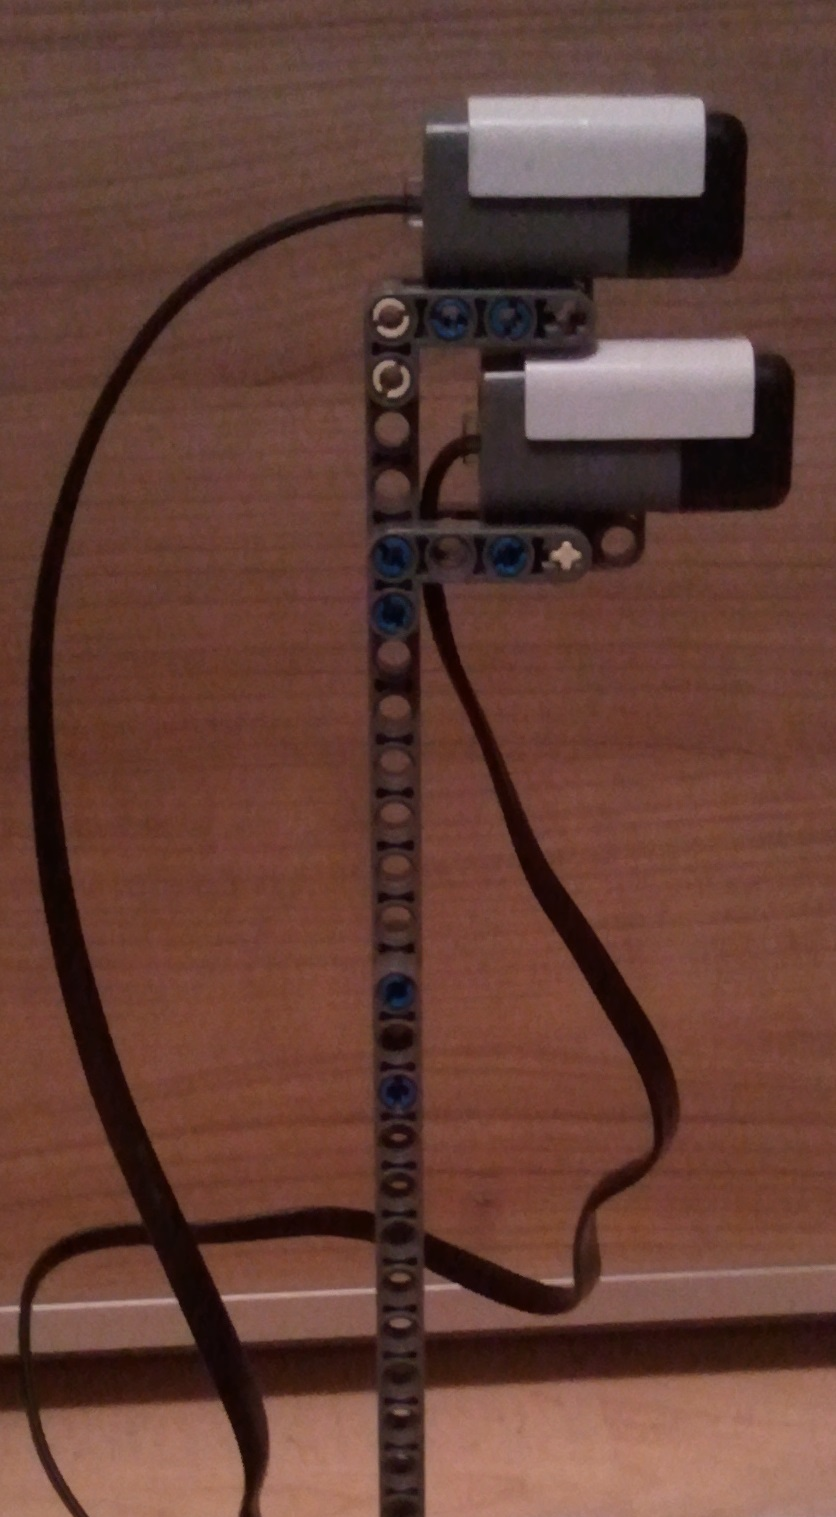
\includegraphics[width=5cm]{images/construction/basis/turm}
\end{capfigure}

Der Turm wurde möglichst nah am Drehpunkt des Roboters befestigt. 

\subsection{Sensoren}
\label{cha:sensoren}
Die Sensoren wurden an der Vorderseite der Basis angebracht. 

\begin{capfigure}[Sensoren]
	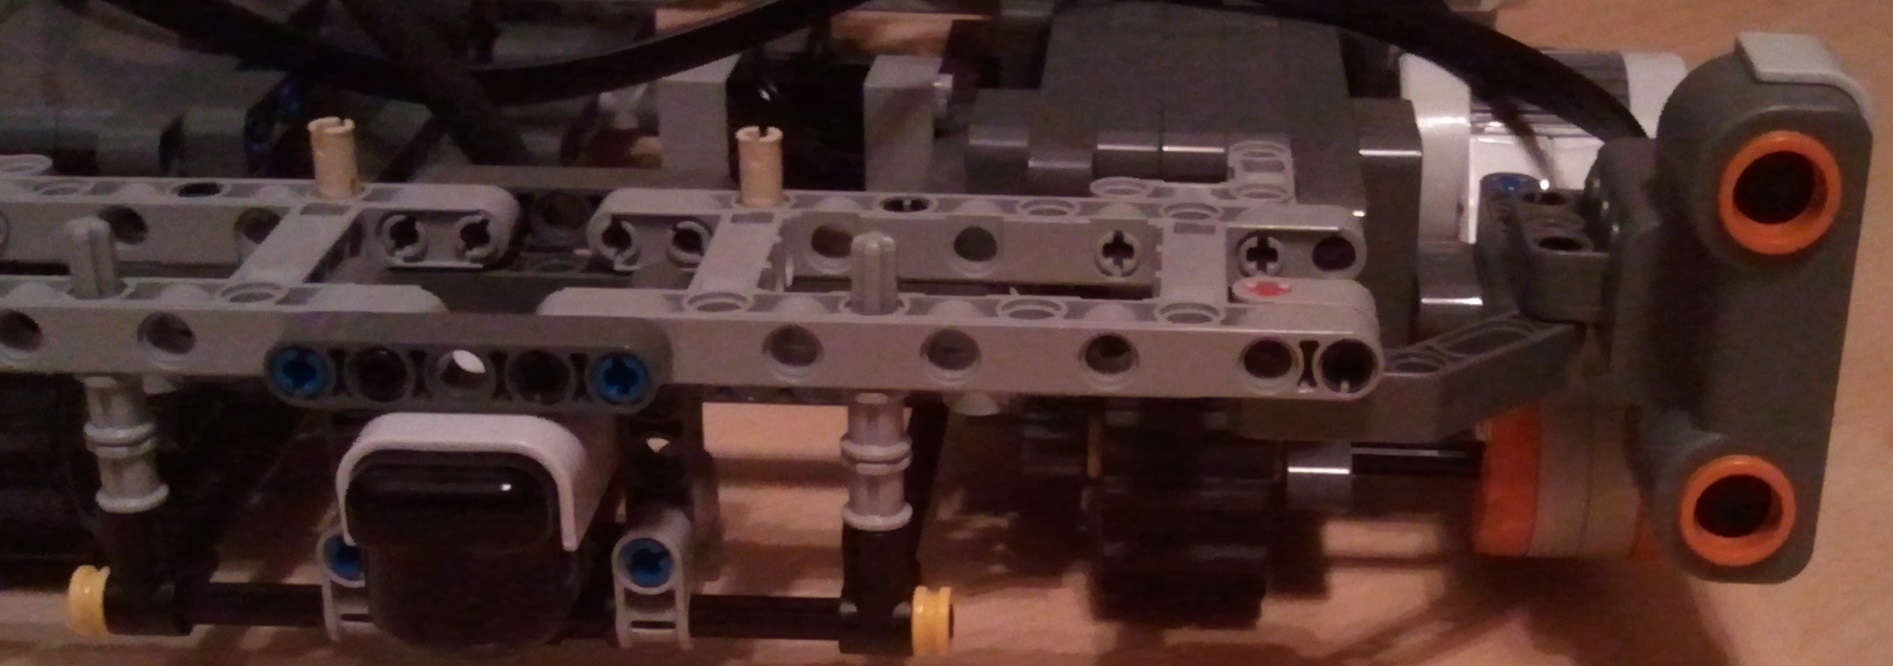
\includegraphics[width=\textwidth]{images/construction/basis/sensoren}
\end{capfigure}

Der \textit{HiTechnic Infrared Seeker} wurde in der Mitte angebracht. Der \textit{Ultraschallsensor} wurde an der linken Seite des \textit{EarthROVERs} angebracht.

\section{Fahrwerk}
\label{cha:fahrwerk}
Das Fahrwerk besteht aus vier Ketten. Auf jeder Seite des \textit{EarthROVERs} befinden sich je zwei Ketten.

\begin{capfigure}[Fahrwerk]
	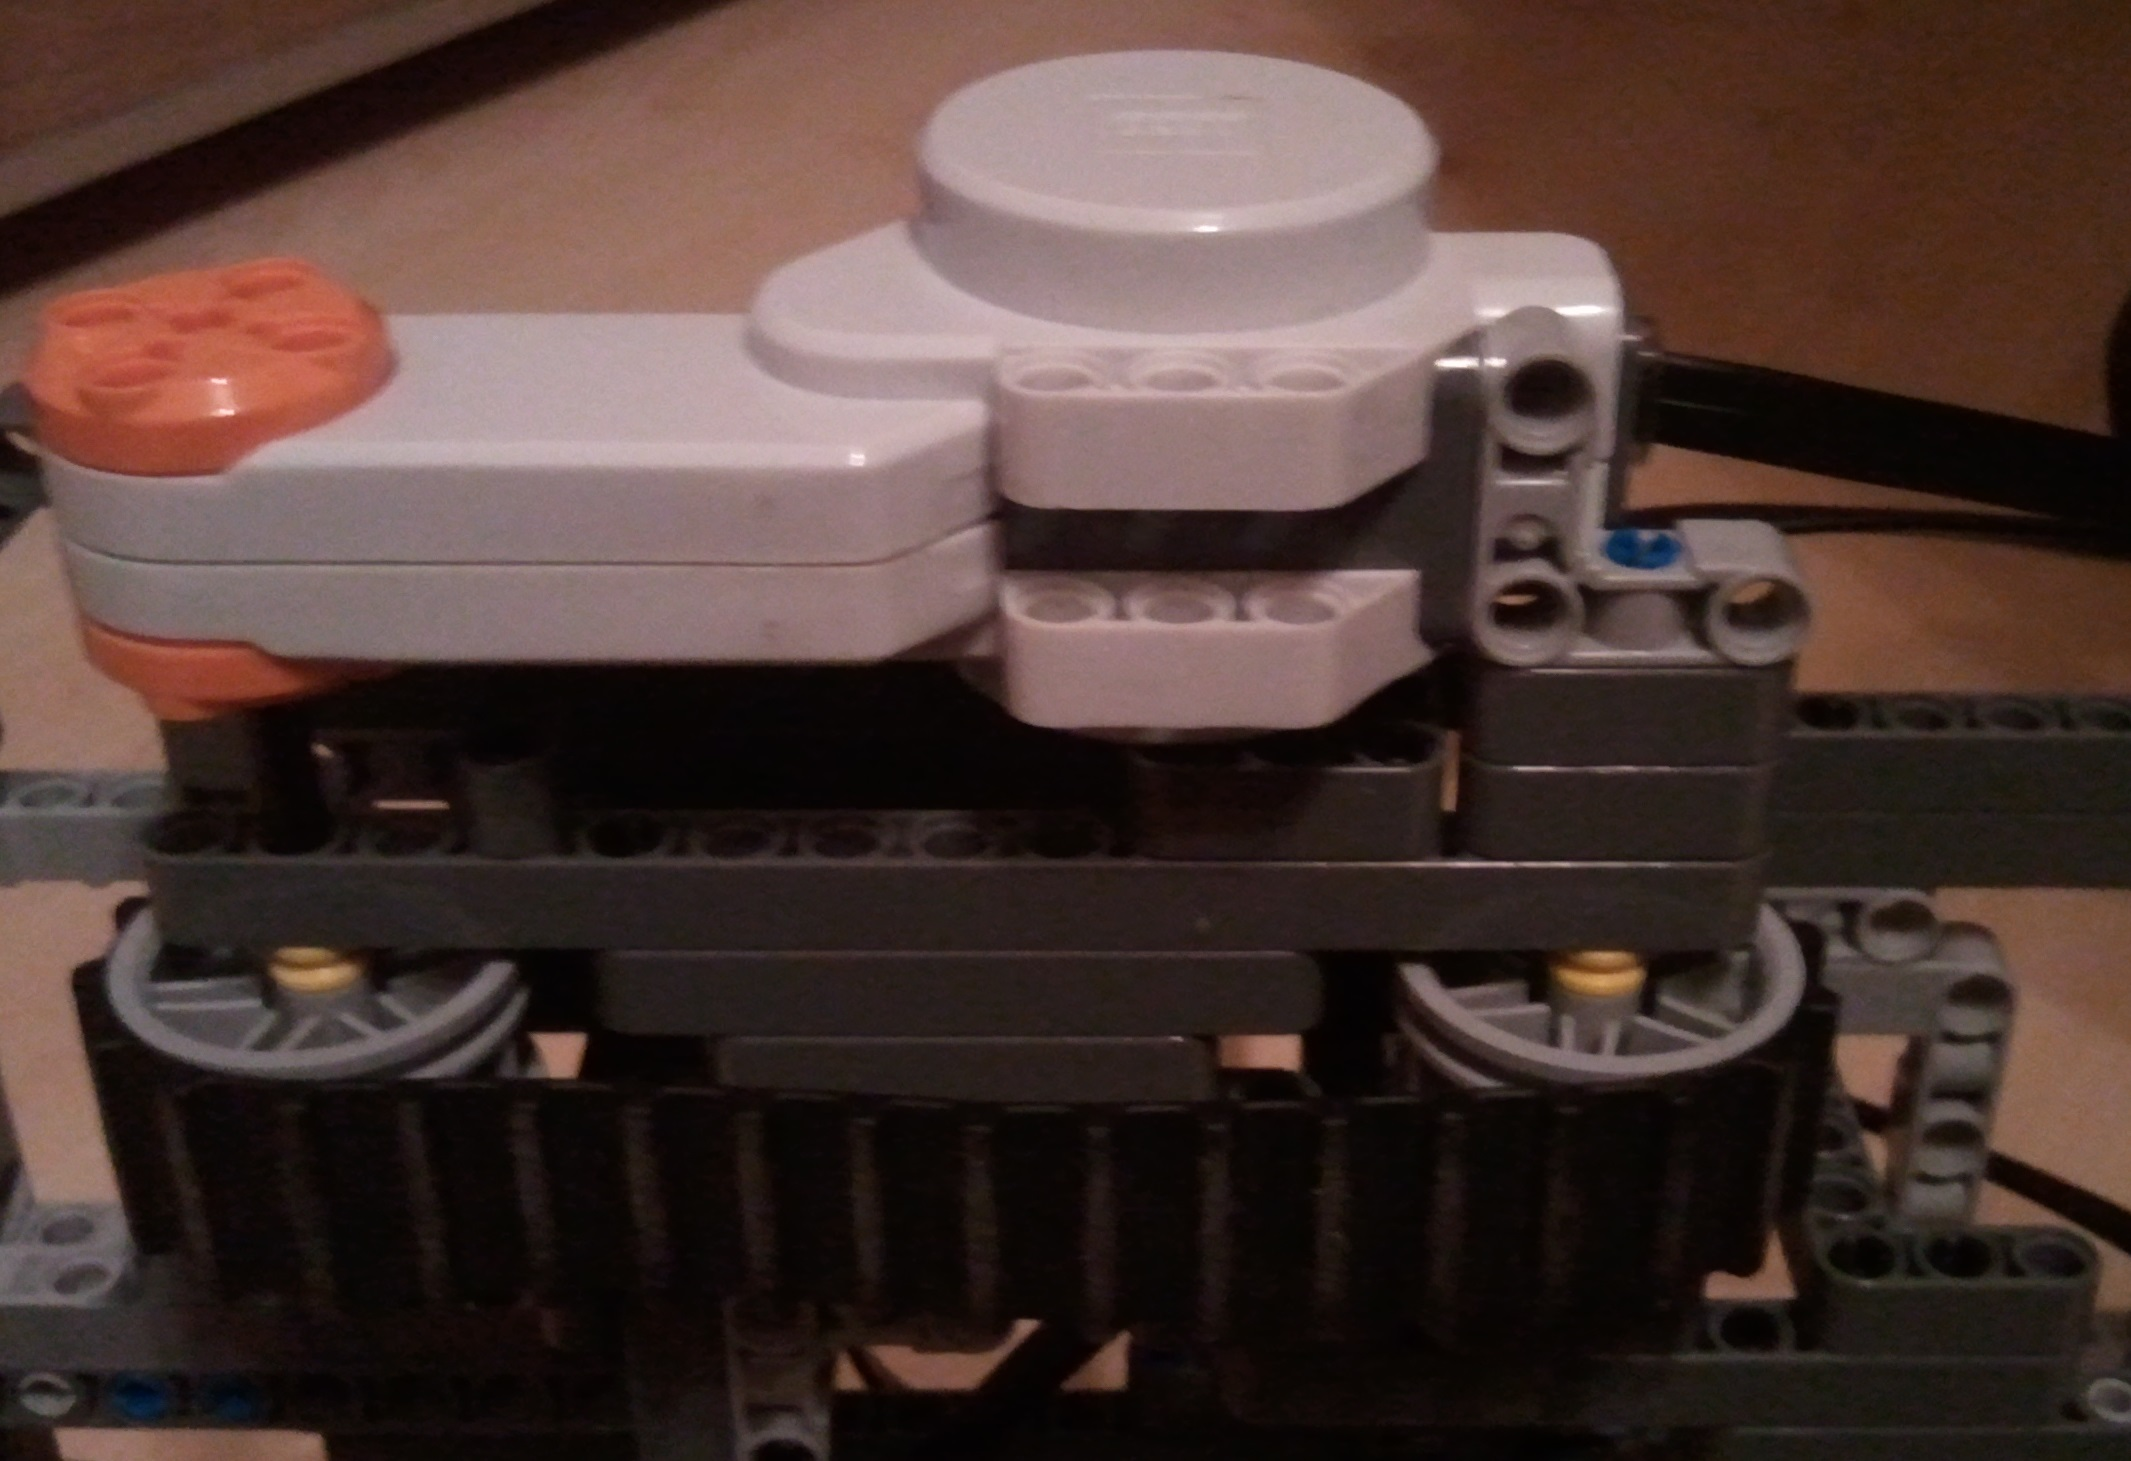
\includegraphics[width=\textwidth]{images/construction/basis/kette}
\end{capfigure}

\section{Greifarm}
Damit der gesuchte Infraotball auch eingefangen werden kann, wird dazu ein Greifarm benötigt. Dieser Greifarm besteht dabei aus 2 Motoren und wird an der Front des Rovers angebracht. Ein Motor dient dabei zum heben und senken des ganzen Armes, der andere Motor dient zum öffnen und schließen des Greifers. Sobald der Rover ab einem Abstand von 9 cm vor dem Ball steht, löst der \textit{HiTechnic Infrared Seeker} das Signal aus um den Arm herunter zufahren und den Ball zu greifen. Ansonsten befindet sich der Greifarm in einem Transportmodus.

\begin{capfigure}[Greifarm im Transportmodus]
	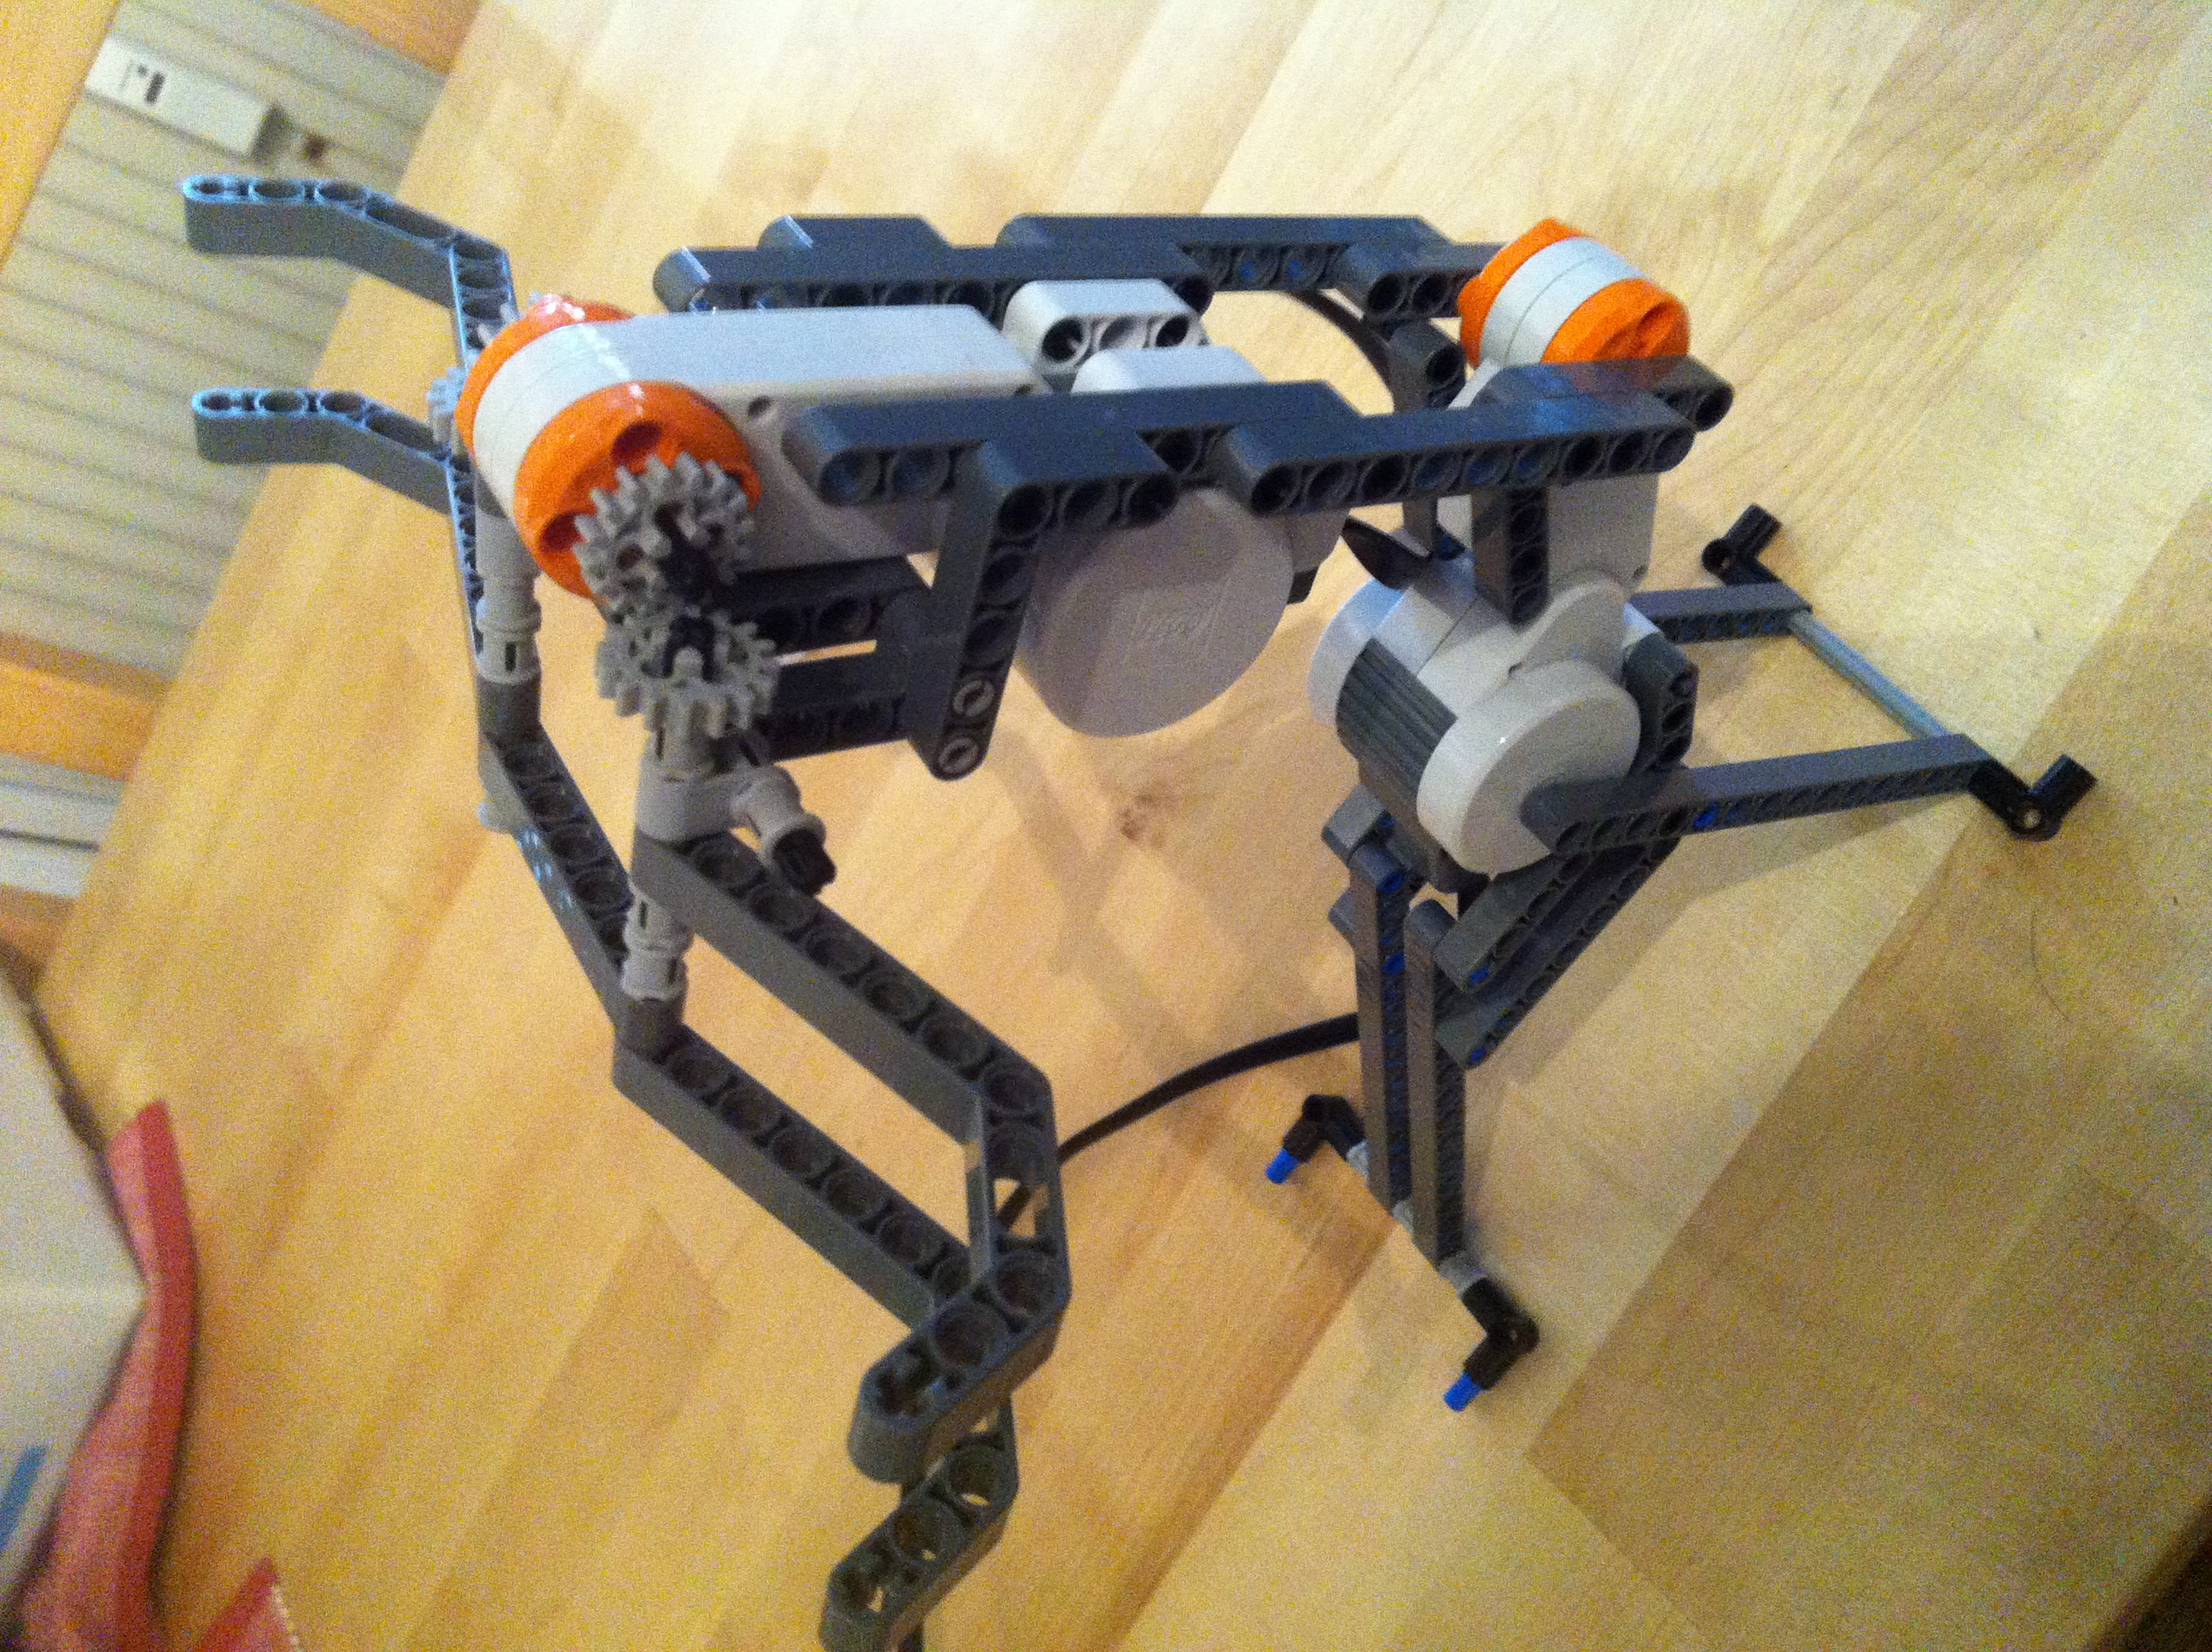
\includegraphics[width=\textwidth]{images/construction/greifarm/Greifarm1}
\end{capfigure}

\begin{capfigure}[Greifarm]
	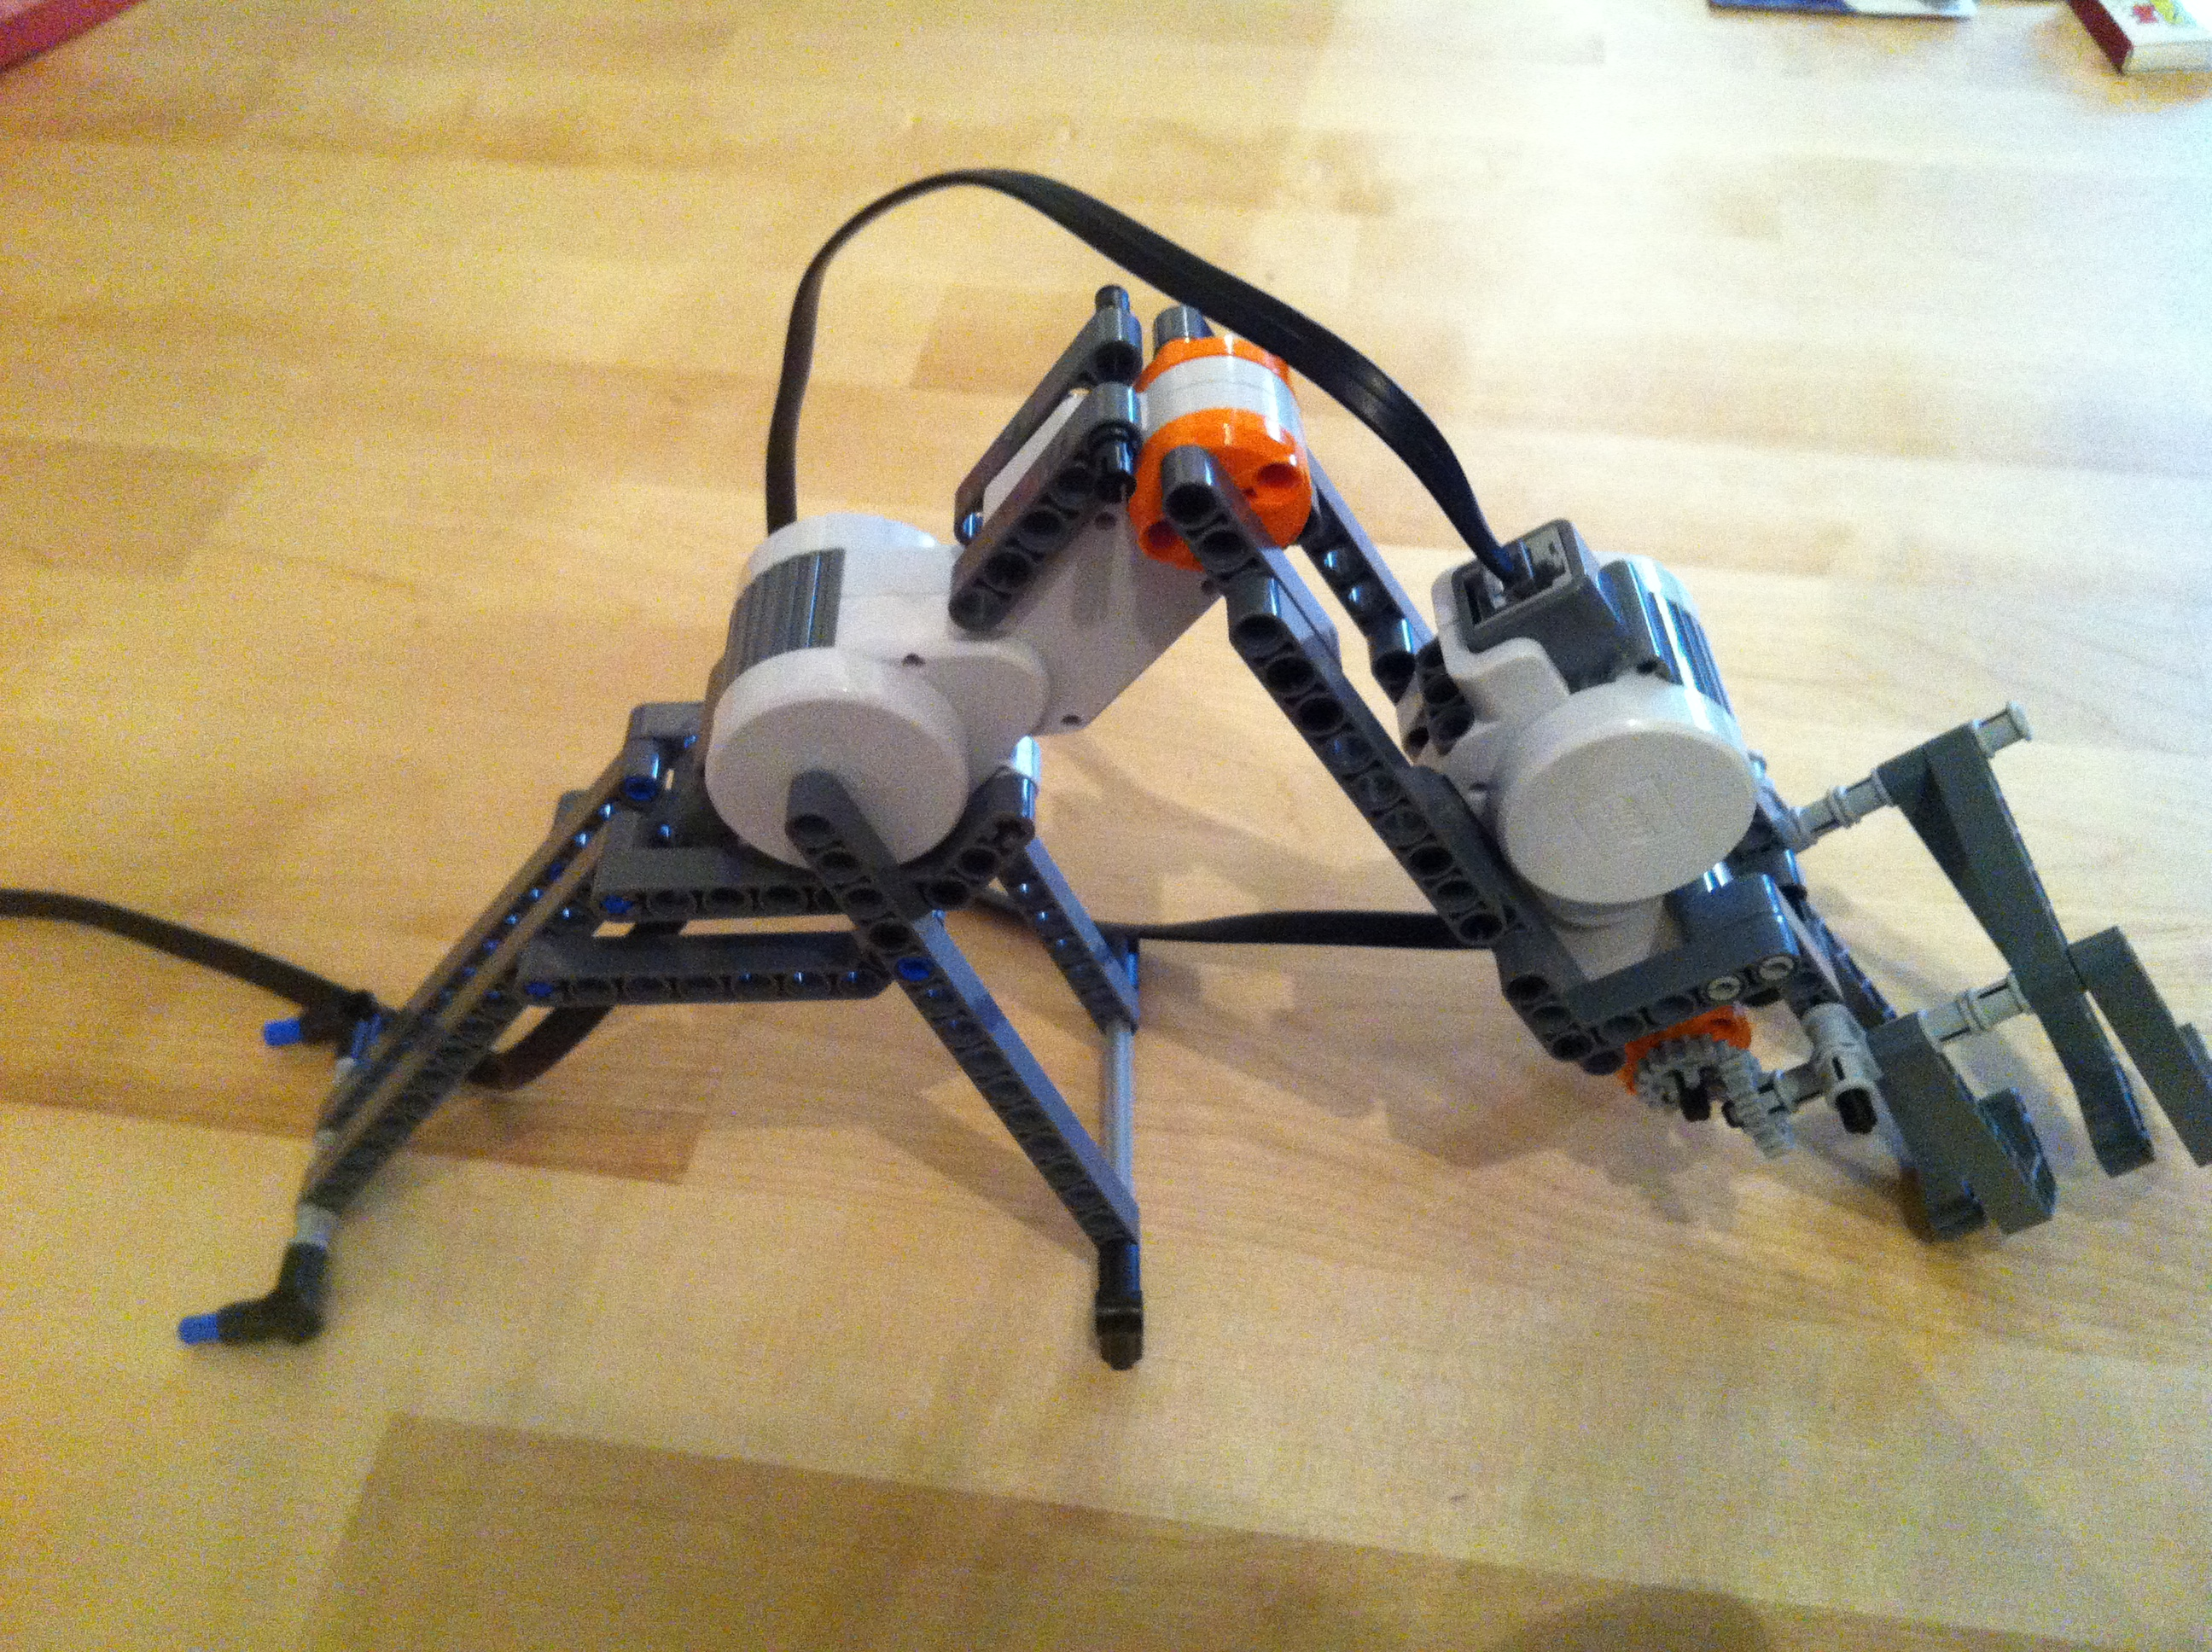
\includegraphics[width=\textwidth]{images/construction/greifarm/Greifarm2}
\end{capfigure}

\begin{capfigure}[Mechanik des Greifers]
	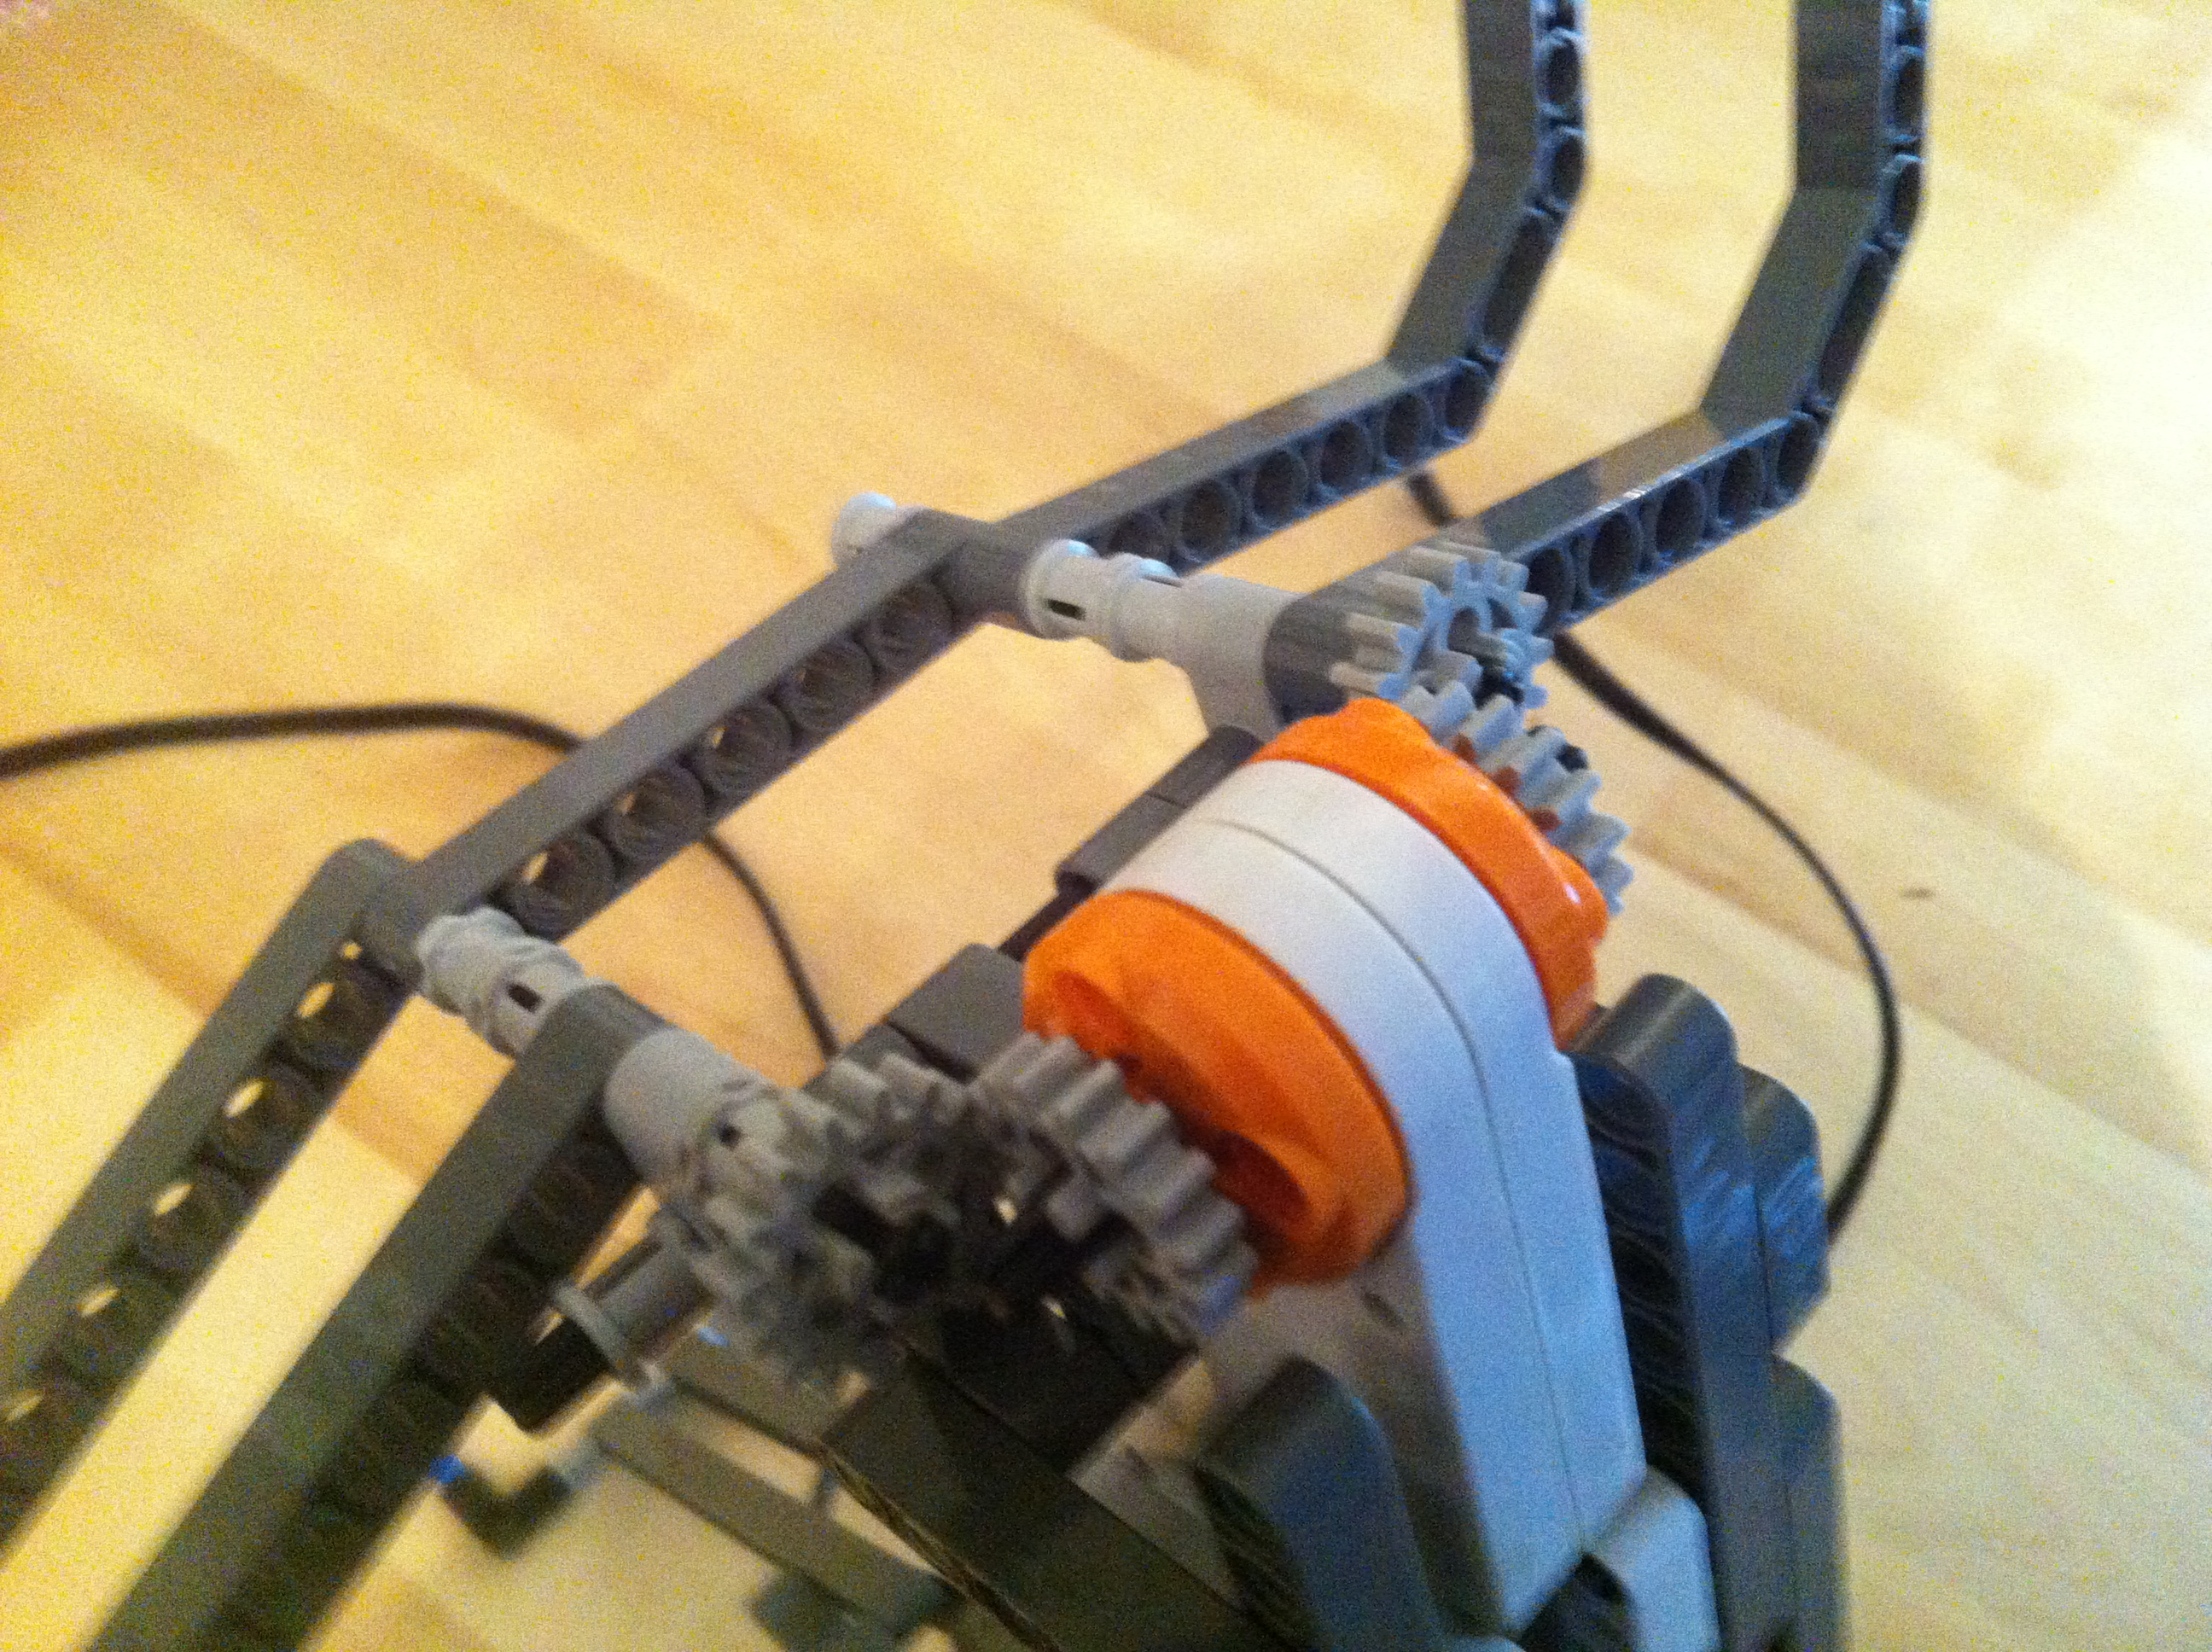
\includegraphics[width=\textwidth]{images/construction/greifarm/Mechanik}
\end{capfigure}